\chapter{DT Convolution}

\section{Review DT LTI systems and superposition property}

Recall the superposition property of LTI systems. If a DT system is LTI then the superposition property holds. Given a system where
\[   
x_i[n] \mapsto y_i[n] \; \forall\; i
\]
then
\[
\sum\limits_{i} a_i x_i[n] \mapsto \sum\limits_{i} a_i y_i[n] 
\]

As in CT we can use superposition to enable a problem reduction strategy in DT systems, where we write the input as a weighted sum of simple signals.  In this lecture, the simple signals are weighted, time shifts of one signal, the DT delta function, $\delta[n]$.

\section{Convolution Sum}

To derive this we start with the sifting property of the DT impulse function (from lecture 3)
\[
\sum\limits_{a}^{b} x[n]\delta[n-n_0] = x[n_0]
\]
for any $a < n_0 < b$. A slight change of variables ($n_0 \rightarrow m$) and limits ($a \rightarrow -\infty$ and $b \rightarrow \infty$) gives:
\[
x[n] = \sum\limits_{m = -\infty}^{\infty} x[m]\delta[n-m]
\]
showing that we can write any DT signal as an infinite sum of weighted and time-shifted impluse functions.

Let $h[n]$ be the DT {\it impulse response}, the output due to the input $\delta[n]$, i.e. $\delta[n] \mapsto h[n]$. Then if the system is time-invariant: $\delta[n-m] \mapsto h[n-m]$ and by superposition, if the input is writen as
\[
x[n] = \sum\limits_{m = -\infty}^{\infty} x[m]\delta[n-m]
\]
then the output is given by
\[
y[n] = \sum\limits_{m = -\infty}^{\infty} x[m]h[n-m] = x[n] * h[n]
\]
This is called the \emph{convolution sum} \index{DT Convolution}.

The significance is similar to that in CT convolution. For a LTI DT system, if I know its impulse response $h[n]$, I can find the response due to \textbf{any} input using convolution. For this reason the impulse response is another way to represent an LTI system.

\section{Graphical View of the Convolution Sum.}

As in CT, let us break the convolution expression down into pieces. In its general form the convolution of two signals $x_1[n]$ and $x_2[n]$ is
\[
x_1[n] * x_2[n] = \sum\limits_{m = -\infty}^{\infty} x_1[m]x_2[n-m]
\]

Suppose $x_1[n]$ and $x_2[n]$ are signals that look like
\begin{center}
  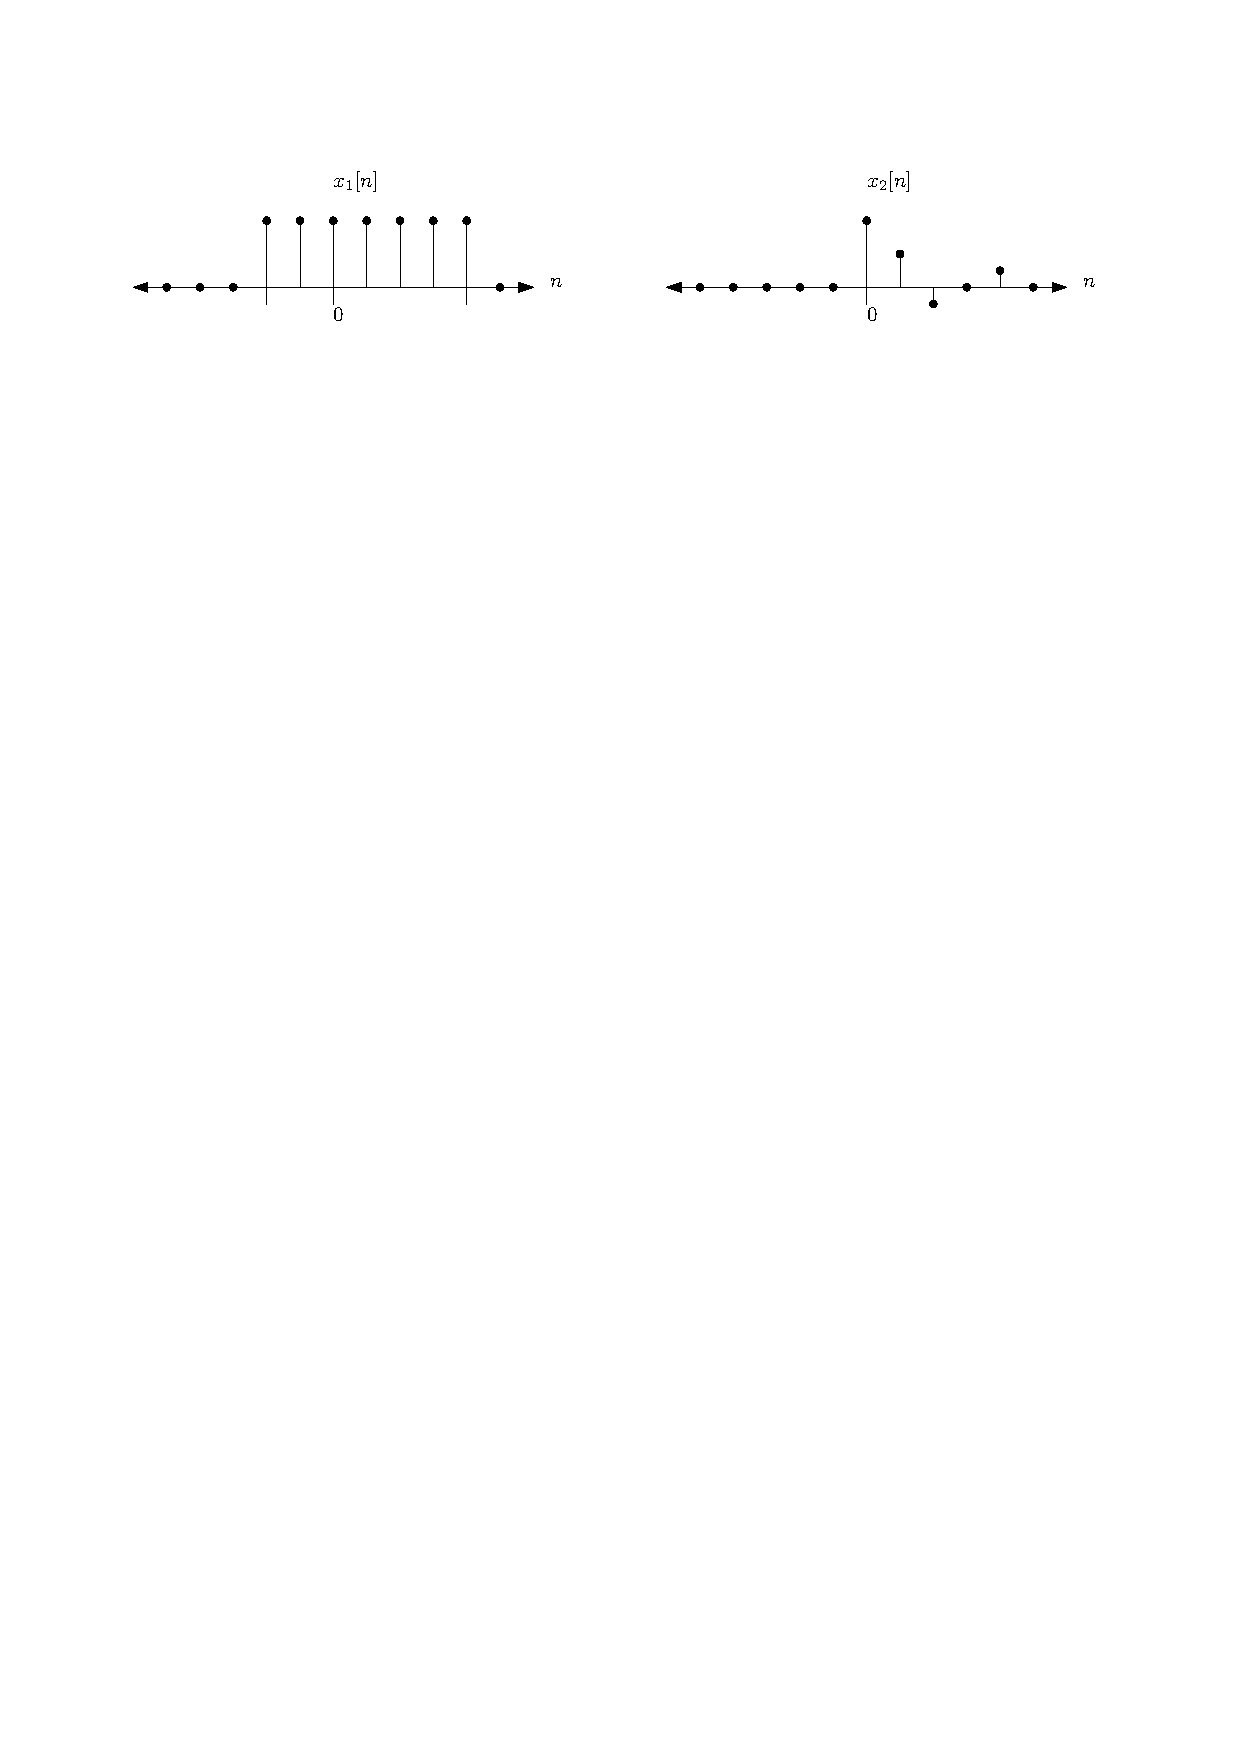
\includegraphics[scale=1]{graphics/dtconvolution-explain1.pdf}
\end{center}

Then $x_1[m]$ and $x_2[-m]$ look like
\begin{center}
  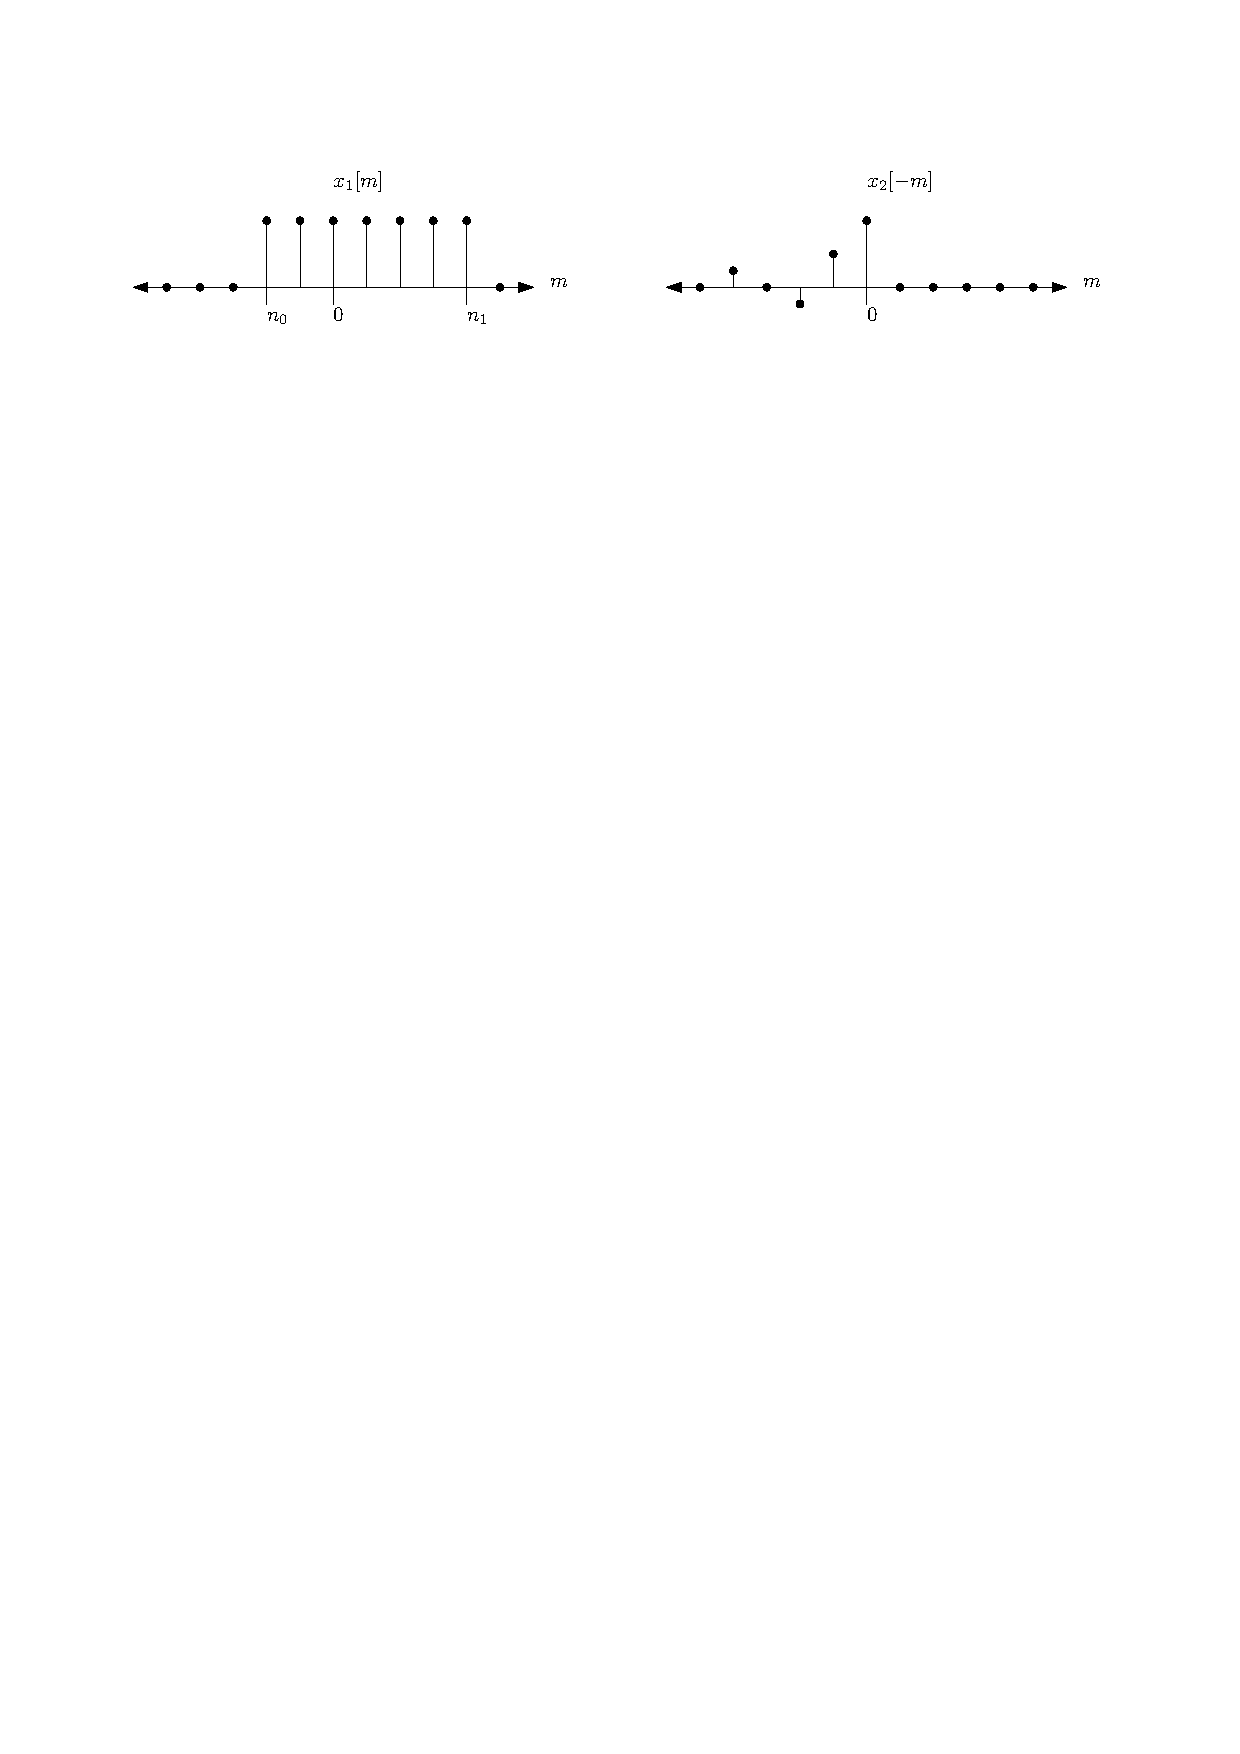
\includegraphics[scale=1]{graphics/dtconvolution-explain2.pdf}
\end{center}

The signal $x_2[n-m]$ is $x_2[-m]$ shifted by $n$ (since $x_2[-m+n]= x_s[n-m]$) and looks like
\begin{center}
  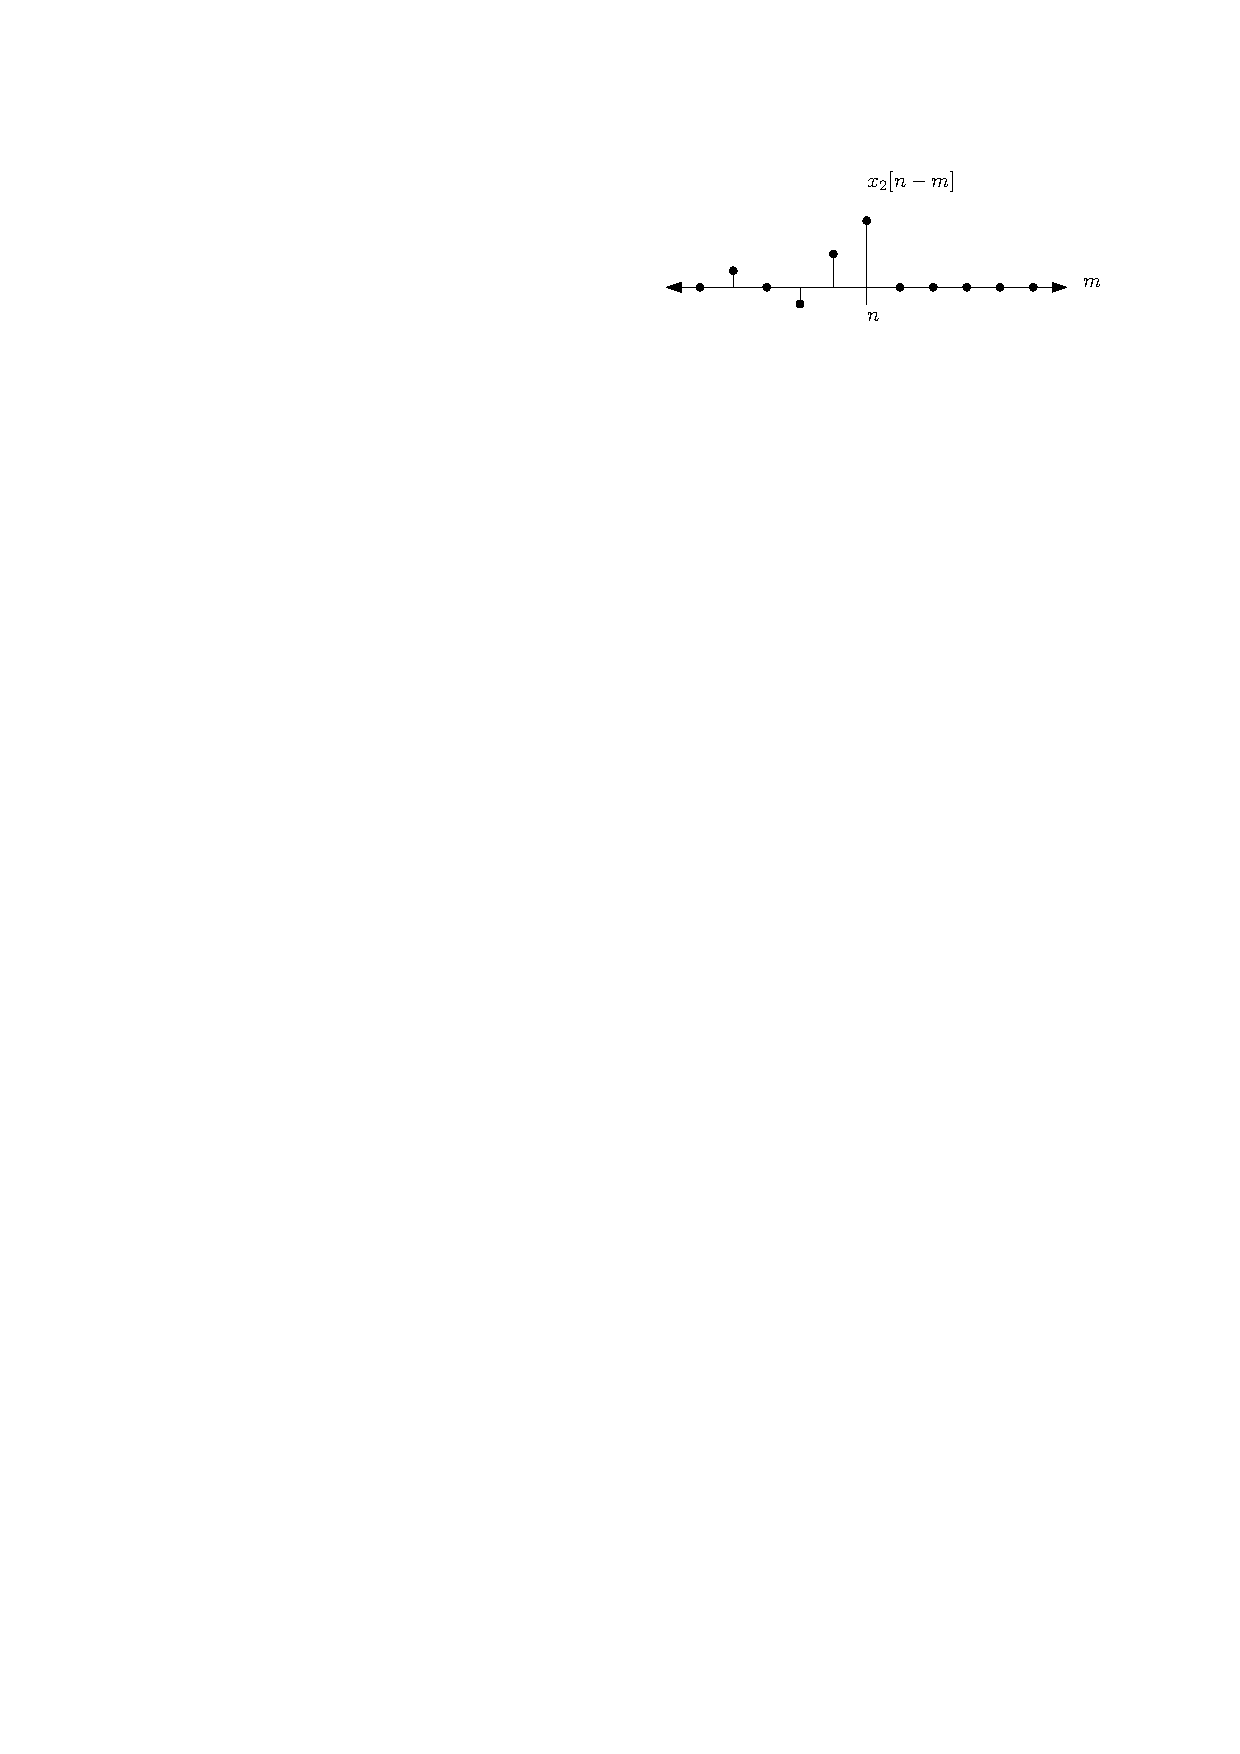
\includegraphics[scale=1]{graphics/dtconvolution-explain3.pdf}
\end{center}

Then the terms of the convolution sum is the product $x_1[m]x_2[n-m]$ whose plot depends of the value of $n$. Some examples, where the individual signals are in grey and their product is in bold:
\begin{center}
  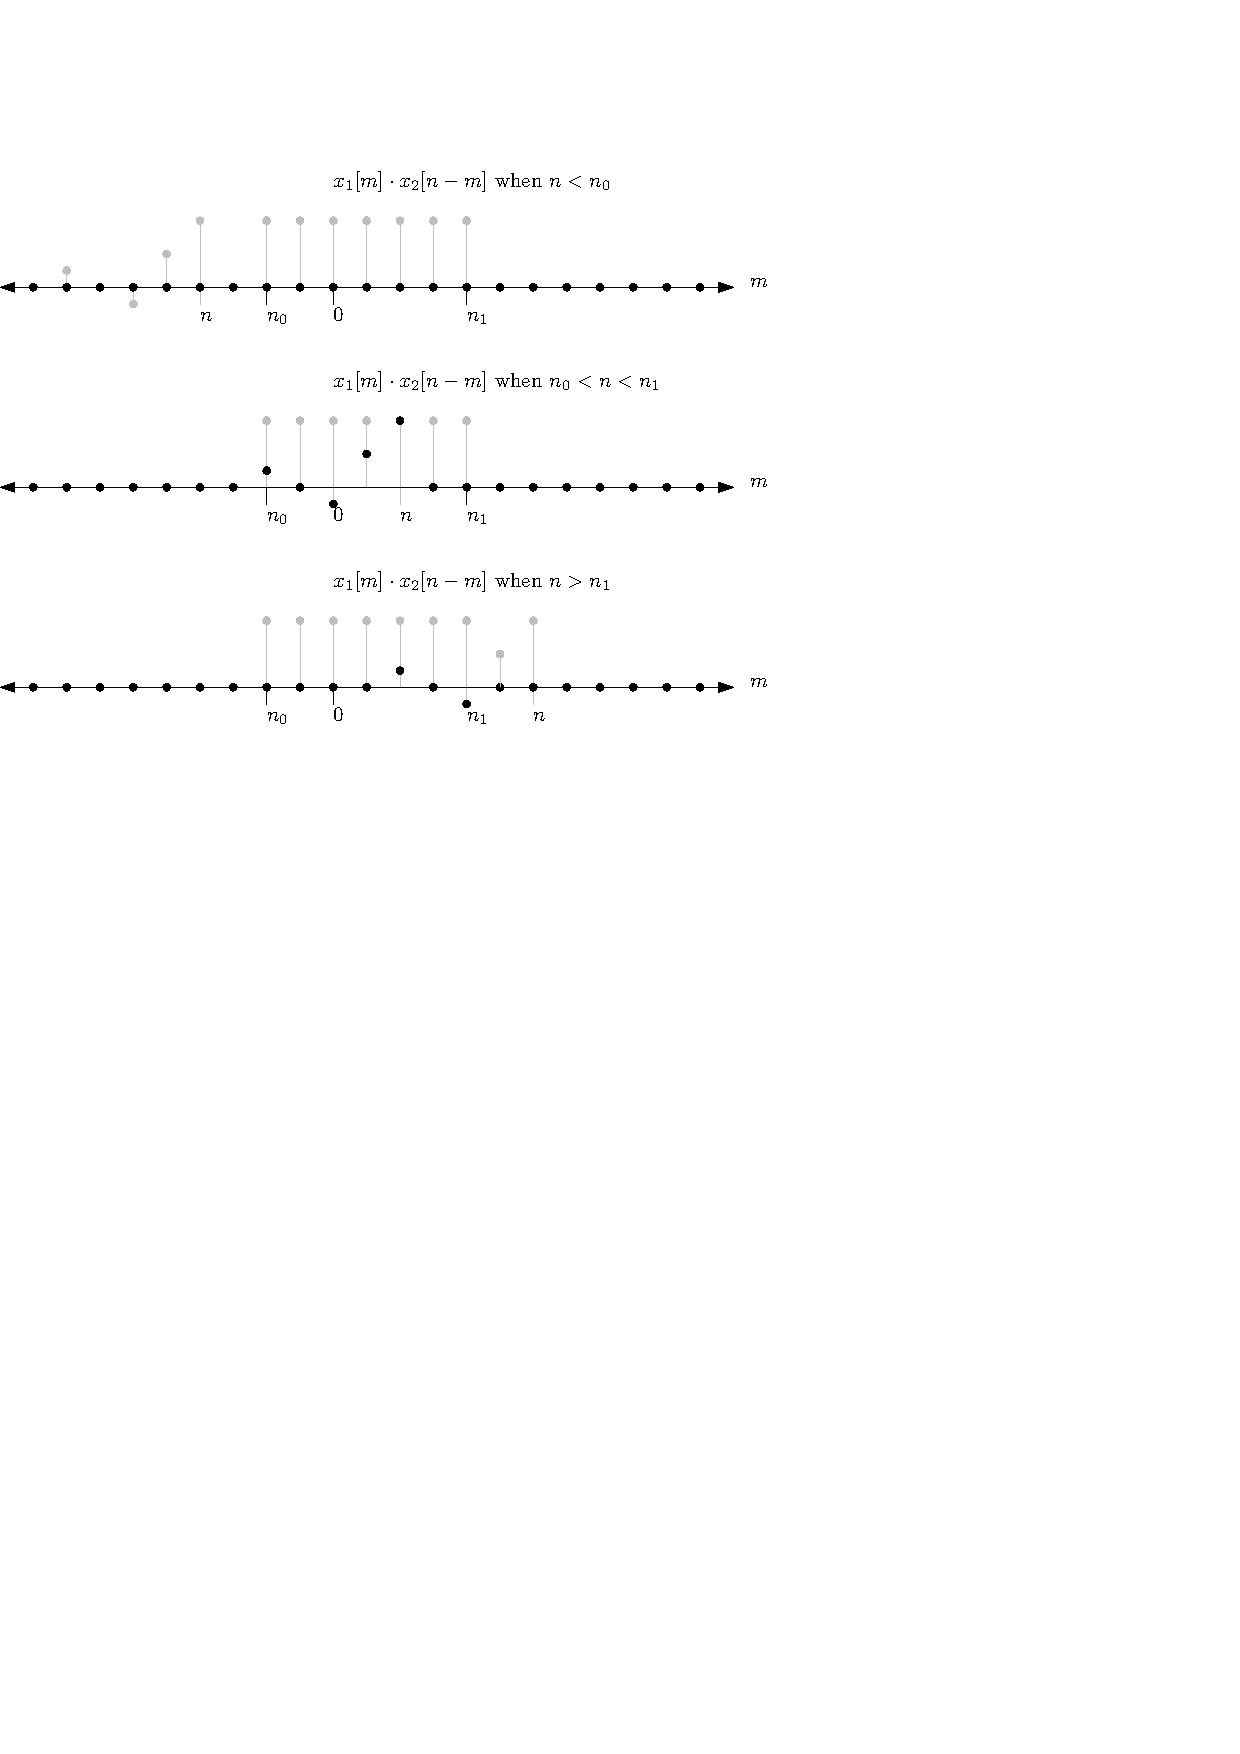
\includegraphics[scale=1]{graphics/dtconvolution-explain4.pdf}
\end{center}

Then convolution is the total sum of the product (bold plots above) for that value of $n$. For the example above we see the sum will be zero for $n$ less than $n_0$ since the two signals do not overlap and their product is zero. For $n_0 \leq n \leq n_1$ the signals overap and the product is non-zero, and the effective bounds of summation are $[n_0,n]$. For $n > n_1$ the signals again overap and the product is non-zero, but the effective bounds of summation are $[n_0,n_1]$. 

\section{DT Convolution of Finite-Length Signals}

For finite-length signals, DT convolution gives us an algorithm to determine their convolution. Suppose the signal $x_1$ is non-zero only over the interval $[N_1,M_1]$, and the signal $x_2$ is non-zero only over the interval $[N_2,M_2]$. The \emph{length} of the signals are $L_1 = M_1-N_1+1$ and $L_2 = M_2-N_2+1$ respectively. The non-zero terms of the convolution sum (when the signals overlap) is then the range $[N_1+N_2,M_1+M_2]$ and the sum can be truncated as:

\[
x_1[n] * x_2[n] = \sum\limits_{m = N_1+N_2}^{M_1+M_2} x_1[m]x_2[n-m]
\]

It is common to shift both signals so that they both start at index $0$ (in order to be represented as arrays in a zero-based index programming language like C or C++), zero-padding them both to have length $L=L_1+L_2-1$ (zero-pad means to just add zero values to the end of the sequence). Then the convolution becomes
\[
y = x_1 * x_2 = \sum\limits_{m = 0}^{L} x_1[m]x_2[n-m]
\]
where the indexing of $x_2$ is modulo the signal length, i.e. $x_2[(n-m) \mbox{ mod } L]$. The resulting signal after convolution, $y$, is also of length $L$, and can then be shifted back to start at $N_1+N_2$.

\begin{example} The following C++ code computes the convolution of the DT signals $\{1,-1,1\}$ and $\{1,1,1,1\}$.
\begin{verbatim}
  const unsigned int L = 6;
  double x1[L] = {1., -1., 1., 0, 0, 0};
  double x2[L] = {1., 1., 1., 1., 0, 0};
  double y[L];

  for(int n = 0; n < L; n++){
    double sum = 0.;
    for(int m = 0; m < L; m++){
      int idx = (L+n-m) % L;
      sum += x1[m]*x2[idx];
    }
    y[n] = sum;
  }
\end{verbatim}
Note that $L_1 = 3$, $L_2 = 4$, so that $L=6$.
$\blacksquare$
\end{example}

An interesting aside, convolution of finite length signals is equivalent to multiplication of two polynomials, where the signal values are the coefficients.

\section{Examples of DT Convolution}

\begin{example} Consider the convolution of two unit step functions:
  \[
  u[n] * u[n] = \sum\limits_{m = -\infty}^{\infty} u[m]u[n-m]
  \]
  Note for $n < 0$ the product of the signals $u[m]$ and $u[n-m]$ is zero as shown in the following figure
  \begin{center}
  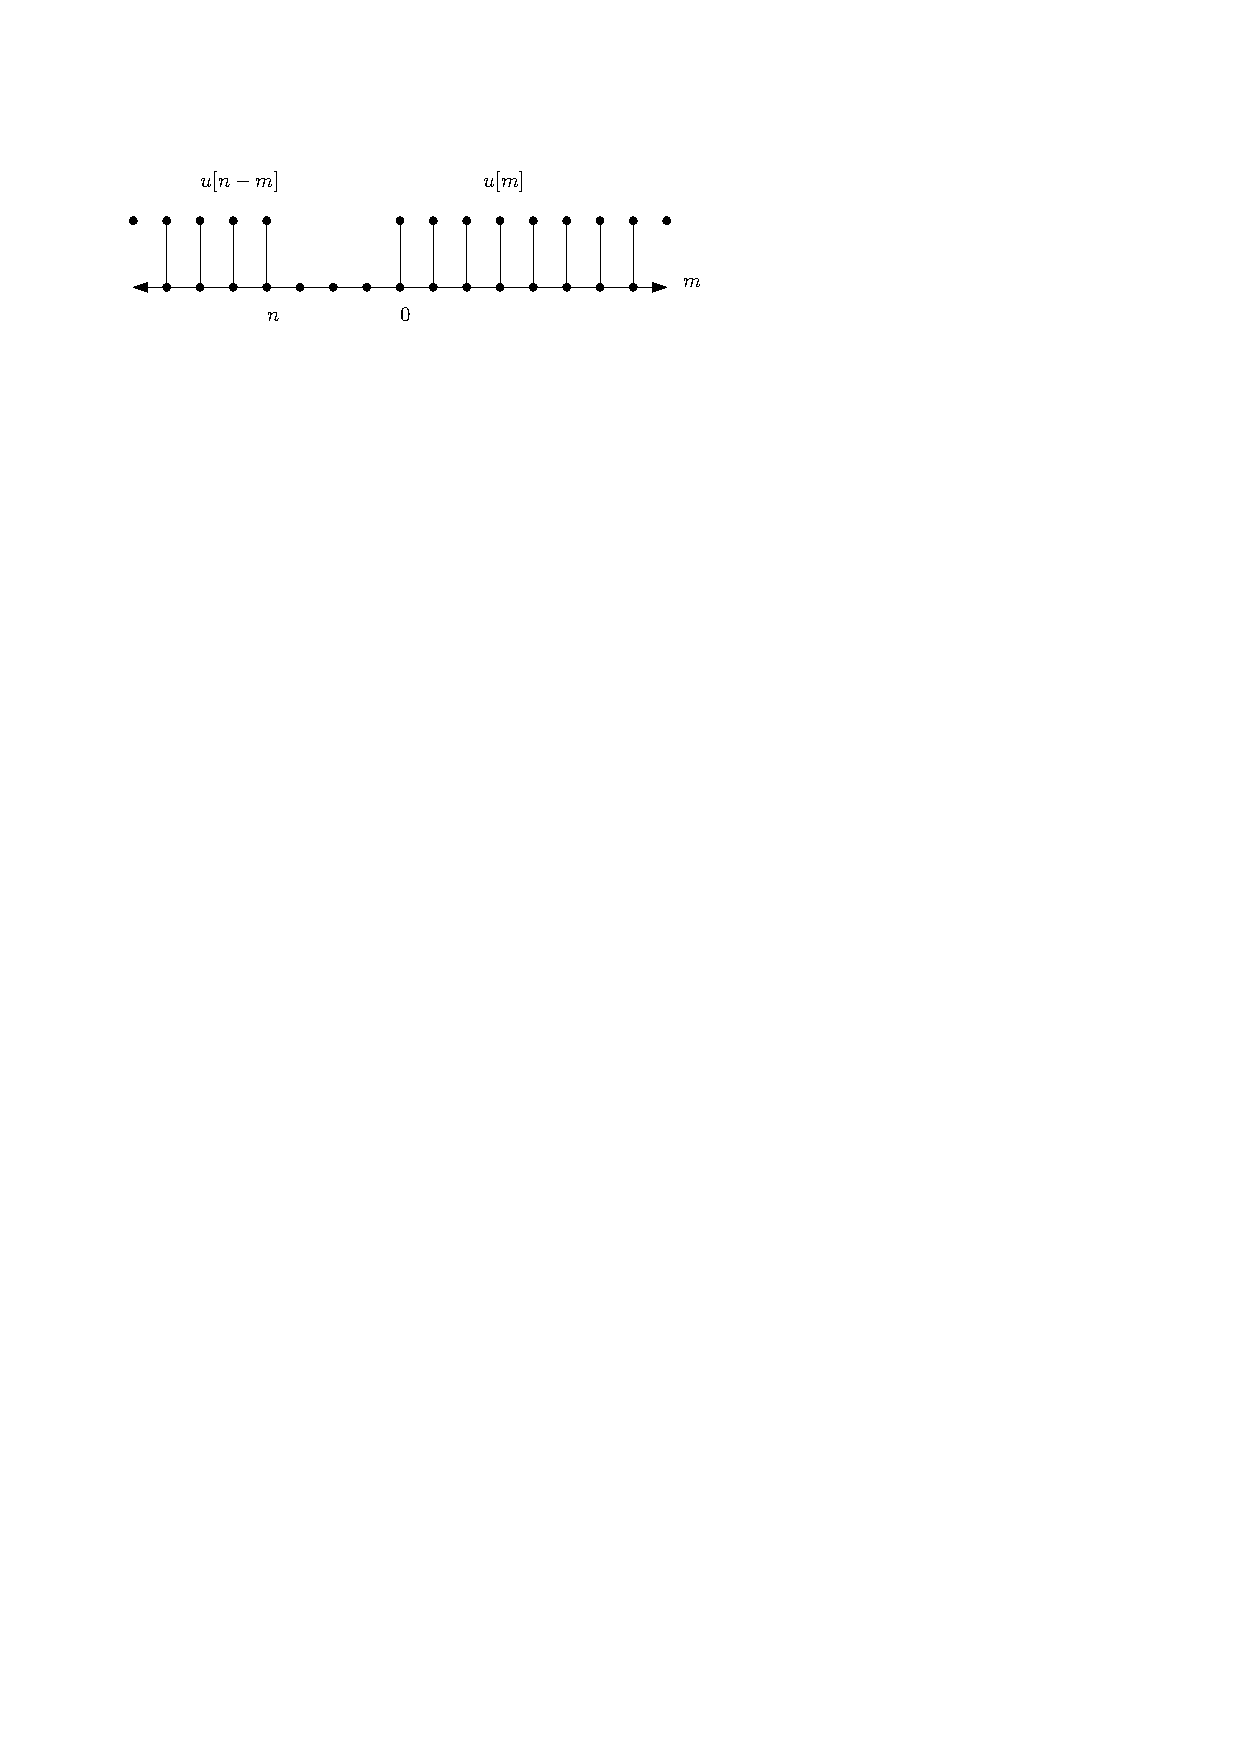
\includegraphics[scale=1]{graphics/dt-step-step-conv.pdf}
  \end{center}
  so that the resulting sum is zero for any $n < 0$. For $n \geq 0$ the signals $u[m]$ and $u[n-m]$ overlap from $0$ to $n$ as shown below
  \begin{center}
    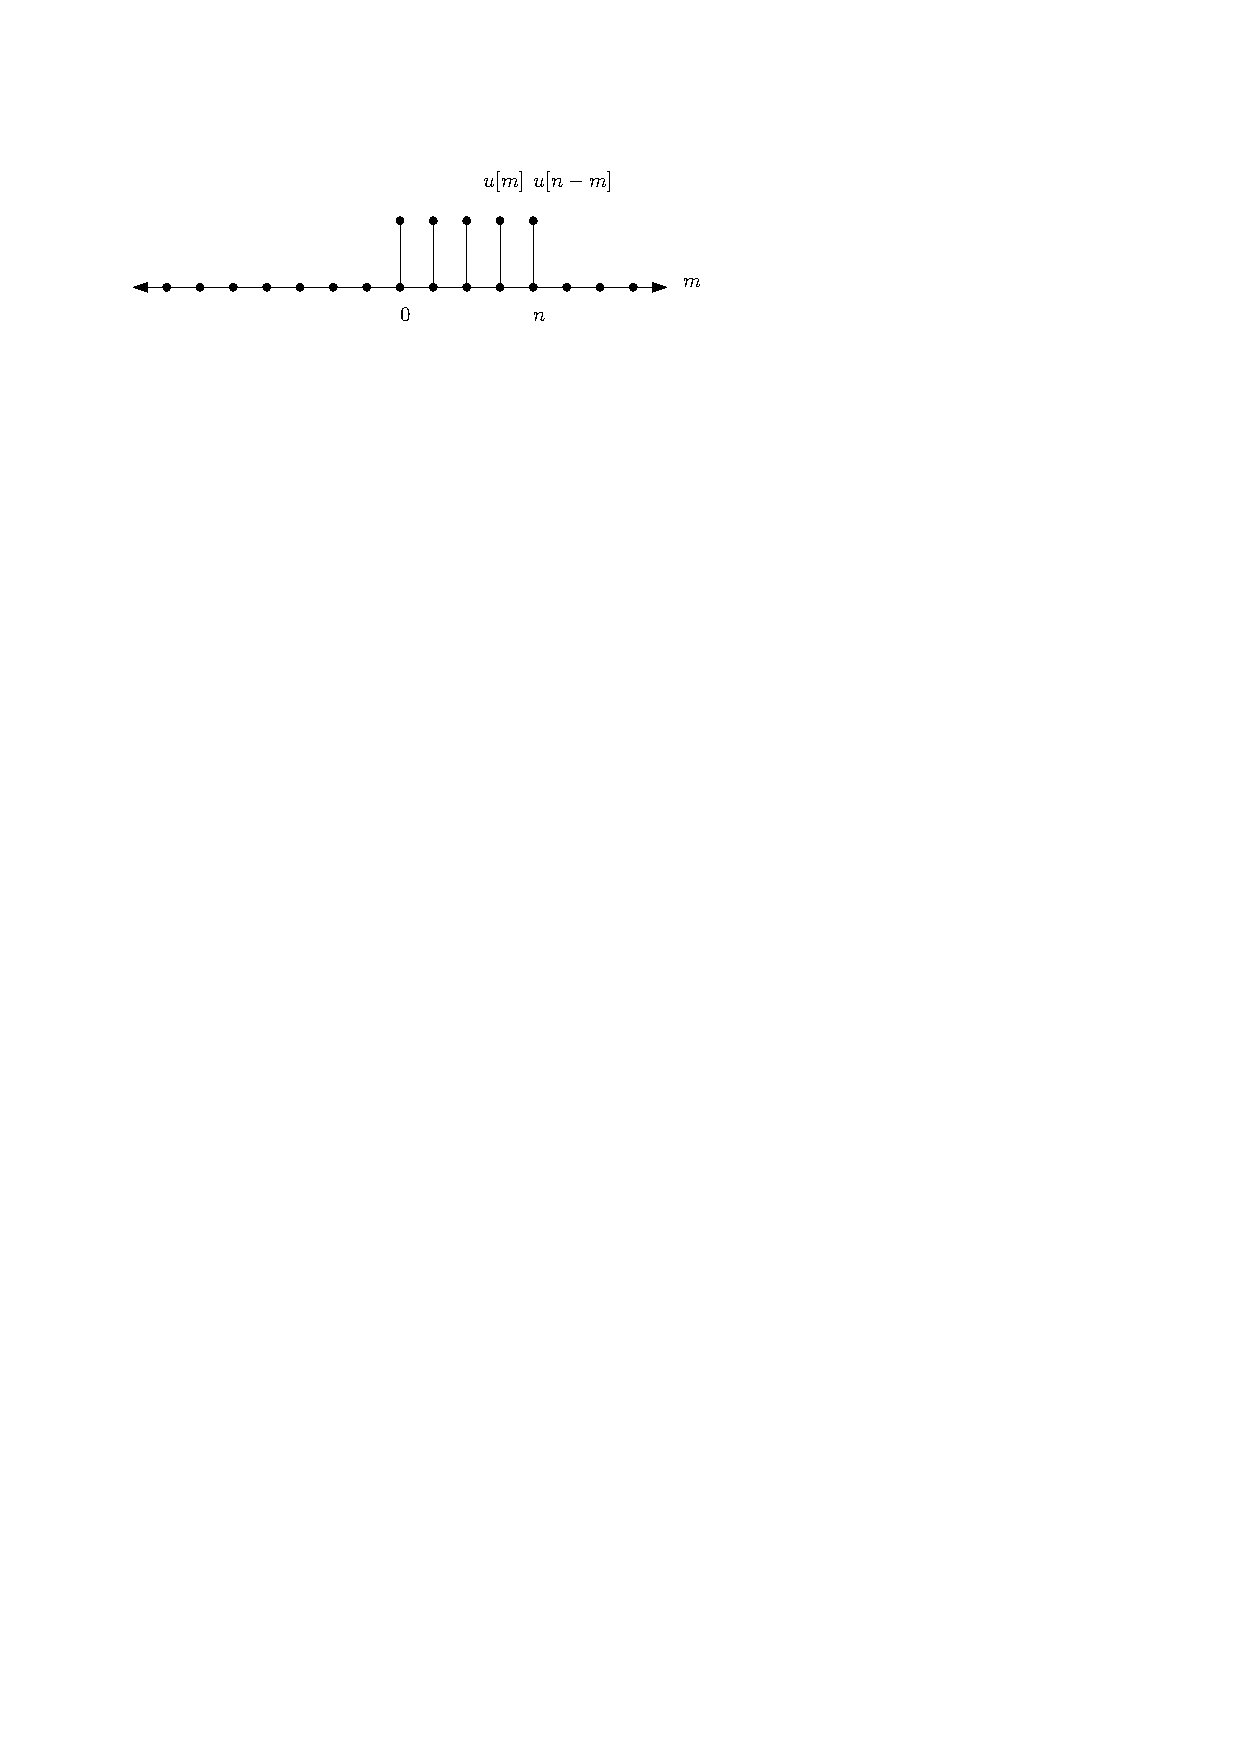
\includegraphics[scale=1]{graphics/dt-step-step-conv2.pdf}
  \end{center}
  and the convolution sum is
  \[
  \sum\limits_{m = 0}^{n} 1 = (n+1)
  \]
  so that
  \[
  u[n] * u[n] = \left\{ \begin{array}{lc}
    0 & n < 0\\
    n+1 & n \geq 0
  \end{array}
  \right.
  \]
  Putting the piecewise result into a single expression gives
  \[
  u[n] * u[n] = (n+1)u[n]
  \]
  $\blacksquare$
\end{example}

\begin{example}
Consider the convolution of a unit step and the function $\gamma^n\,u[n]$ for some constant $\gamma \neq 1$:
  \[
  \gamma^n\, u[n] * u[n] = \sum\limits_{m = -\infty}^{\infty} \gamma^{m}u[m]u[n-m]
  \]
  Since both signals are multiplied by a step, the product of $\gamma^{m}u[m]u[n-m]$ is non-zero only for $0 \leq m \leq n$ (for the same reason as in the previous example). Thus for $n \geq 0$ the convolution sum is:
  \[
  \sum\limits_{m = 0}^{n} \gamma^{m} = \frac{\gamma^{n+1}-1}{\gamma-1} = \frac{1-\gamma^{n+1}}{1-\gamma}
  \]
  Putting the two piecewise results together gives
  \[
  \gamma^n\, u[n] * u[n] = \frac{1-\gamma^{n+1}}{1-\gamma}\,u[n]
  \]
  $\blacksquare$
\end{example}
\begin{example} Consider the convolution of an arbitrary signal $x[n]$ with the impulse function
  \[
  x[n] * \delta[n] = \sum\limits_{m = -\infty}^{\infty} x[m]\delta[n-m]
  \]
  By the sifting property we get
  \[
  \sum\limits_{m = -\infty}^{\infty} x[m]\delta[n-m] = x[n]
  \]
  Thus the convolution with the impulse gives back the same signal (the $\delta$ is the \emph{identity} signal). $\blacksquare$
\end{example}

\noindent Table \ref{table:dtconv} lists several DT convolution results.

\section{Properties of DT Convolution}
There are several useful properties of convolution. We do not prove these here, but it is not terribly difficult to do so. Given signals $x_1[n]$, $x_2[n]$, and $x_3[n]$:

\begin{description}
\item [Commutative Property] The ordering of the signals does not matter.
  \[
x_1[n] * x_2[n] = x_2[n] * x_1[n]
  \]
\item [Distributive Propery] Convolution is distributed over addition.
  \[
  x_1[n] * \left(x_2[n] + x_3[n]\right) = \left(x_1[n] * x_2[n] \right) + \left(x_1[n] * x_3[n] \right) 
  \]
\item [Associative Property] The order of convolution does not matter.
    \[
  x_1[n] * \left(x_2[n] * x_3[n]\right) = \left(x_1[n] * x_2[n] \right) * x_3[n] 
  \]
\item [Index Shift] Given $x_3[n] = x_1[n] * x_2[n]$ then for index shifts $m_1, m_2 \in \mathbb{R}$
  \[
  x_1[n-m_1] * x_2[n-m_2] = x_3[n-m_1 - m_2]
  \]
\item [Multiplicative Scaling] Given $x_3[n] = x_1[n] * x_2[n]$ then for constants $a,b \in \mathbb{C}$
  \[
  \left(a\, x_1[n]\right) * \left(b\, x_2[n]\right) = a\, b\, x_3[n]
  \]
\end{description}

These properties can be used in combination with a table like that above to compute the convolution of a wide variety of signals without evaluating the summations.

\begin{example} Consider the convolution of the causal DT pulse of length $N$, $x_1[n] = u[n] - u[n-N]$, and the signal $x_2[n] = \left( \frac{1}{2}\right)^nu[n]$.

  \begin{align*}
    x_1[n] * x_2[n] &= \left( u[n] - u[n-N]\right) * \left( \left( \frac{1}{2}\right)^nu[n] \right)\\
    &= \left( u[n] \right) * \left( \left( \frac{1}{2}\right)^nu[n] \right) - \left( u[n-N]\right) * \left( \left( \frac{1}{2}\right)^nu[n] \right) \mbox{ using distributive property}\\
    &= \frac{1-\left(\frac{1}{2}\right)^{n+1}}{1-\left(\frac{1}{2}\right)}u[n] - \frac{1-\left(\frac{1}{2}\right)^{n+1}}{1-\left(\frac{1}{2}\right)}u[n] \Big|_{n\rightarrow n-N} \mbox{ from Table row 2 and index shift property}\\
    &= \frac{1-\left(\frac{1}{2}\right)^{n+1}}{\left(\frac{1}{2}\right)}u[n] - \frac{1-\left(\frac{1}{2}\right)^{n-N+1}}{\left(\frac{1}{2}\right)}u[n-N]\\
    &= \frac{1-\left(\frac{1}{2}\right)^{n+1}}{\left(\frac{1}{2}\right)}u[n] - \frac{1-\left(\frac{1}{2}\right)^{-N}\left(\frac{1}{2}\right)^{n+1}}{\left(\frac{1}{2}\right)}u[n-N]\\
    &= 2\left(1-\left(\frac{1}{2}\right)^{n+1}\right)u[n] - 2\left(1-\left(\frac{1}{2}\right)^{-N}\left(\frac{1}{2}\right)^{n+1} \right)u[n-N]\\
    &= \left(2-\left(\frac{1}{2}\right)^{n}\right)u[n] - \left(2-\left(\frac{1}{2}\right)^{-N}\left(\frac{1}{2}\right)^{n} \right)u[n-N]
  \end{align*}
$\blacksquare$
\end{example}

